\documentclass{article}
\usepackage{style}
\begin{document}
\maketitle
\tableofcontents
\section{Introducción}
El algoritmo genético enfatiza la importancia de la cruza y la mutación, al igual que la selección probabilistica.
En esta práctica se implementó la selección por torneo:
\begin{itemize}
	\item Generar aleatoriamente una población inicial.
	\item Calcular la aptitud de cada individuo.
	\item Seleccionar probabilisticamente con base en la aptitud.
	\item Aplicar cruza y mutación para generar la siguiente población.
	\item Ciclar hasta que las condiciones finales se cumplan.
\end{itemize}
\newpage
\section{Contenido}
\subsection{Algoritmo con 10 generaciones}
\begin{figure}[h!]
	\centering
	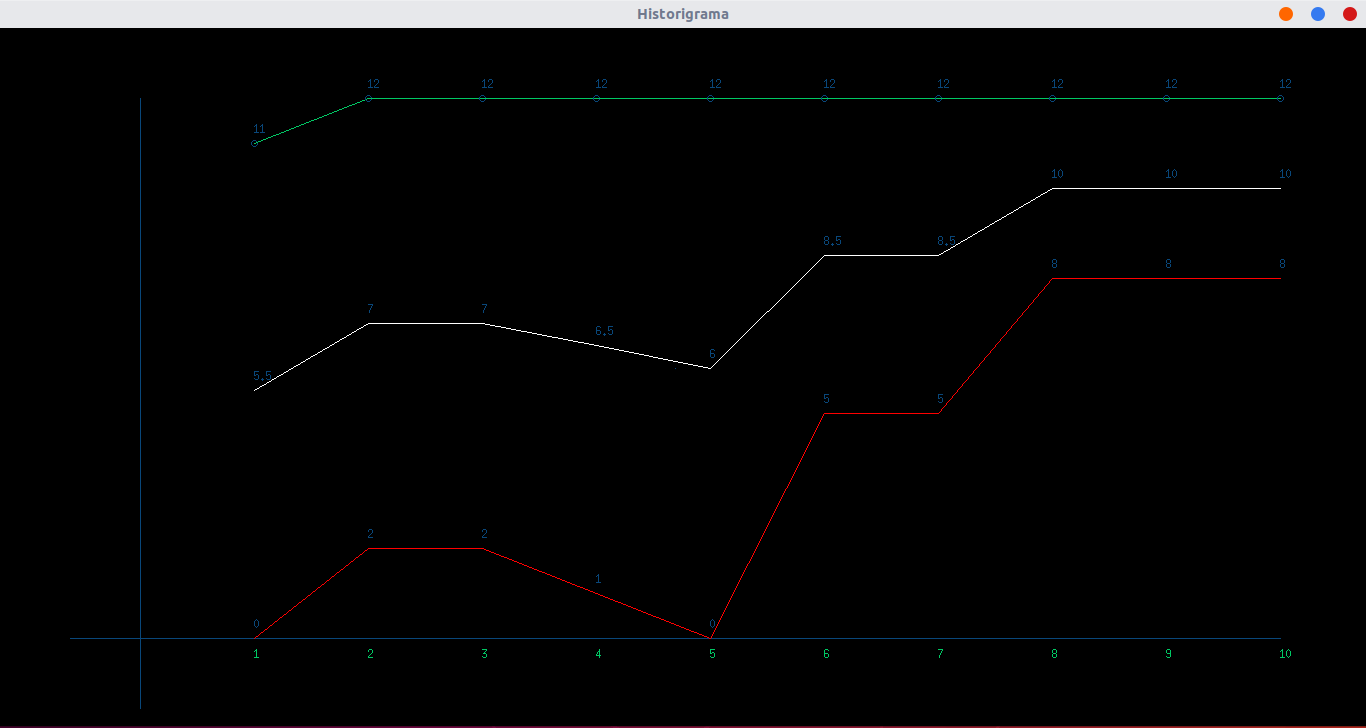
\includegraphics[scale=.3]{10gen}
\end{figure}
\newpage
\subsection{Algoritmo con 30 generaciones}
\begin{figure}[h!]
	\centering
	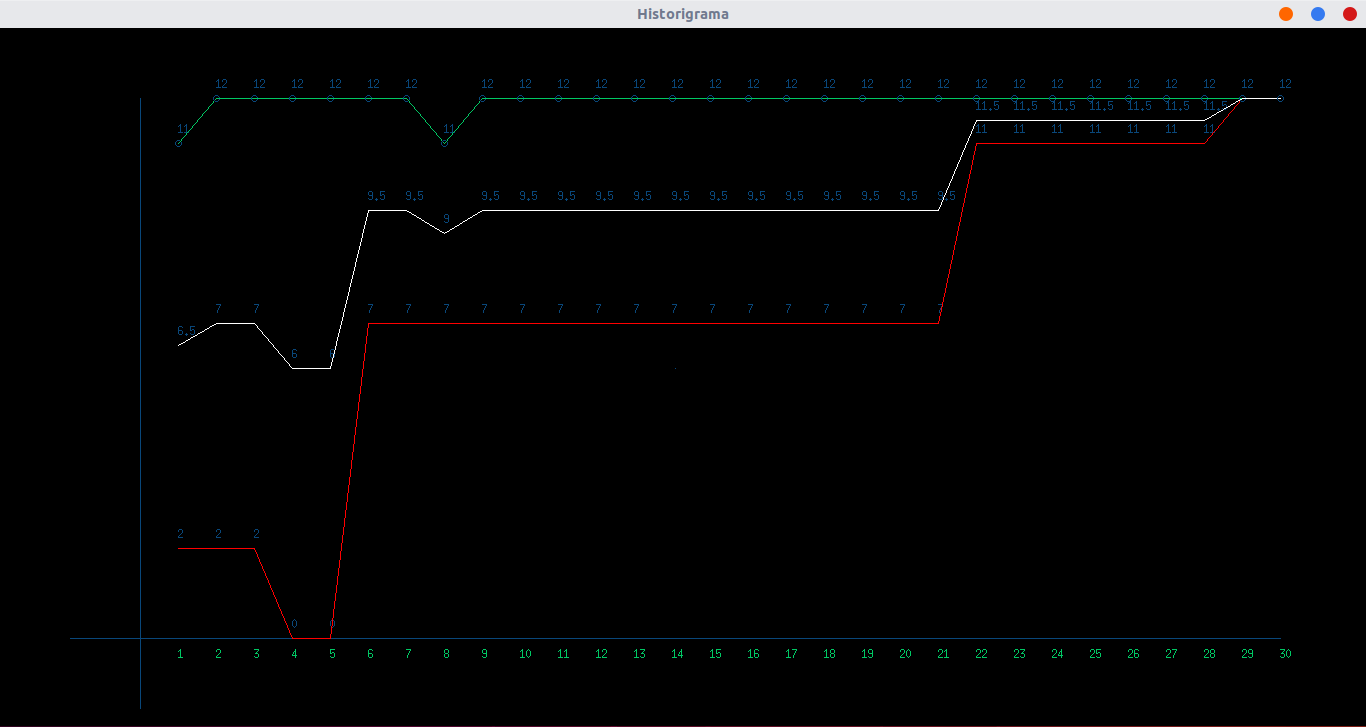
\includegraphics[scale=.3]{30gen}
\end{figure}
\newpage
\subsection{Algoritmo con 50 generaciones}
\begin{figure}[h!]
	\centering
	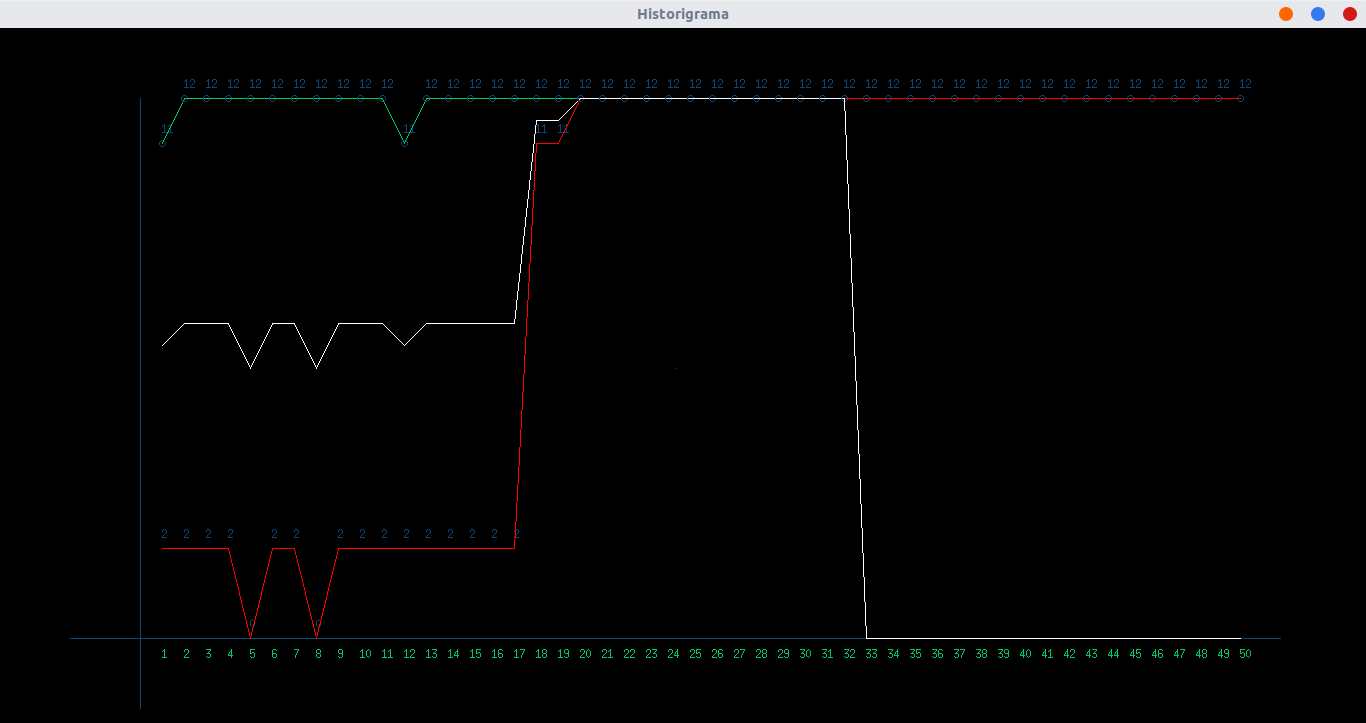
\includegraphics[scale=.3]{50gen}
\end{figure}
\newpage
\subsection{Algoritmo con 100 generaciones}
\begin{figure}[h!]
	\centering
	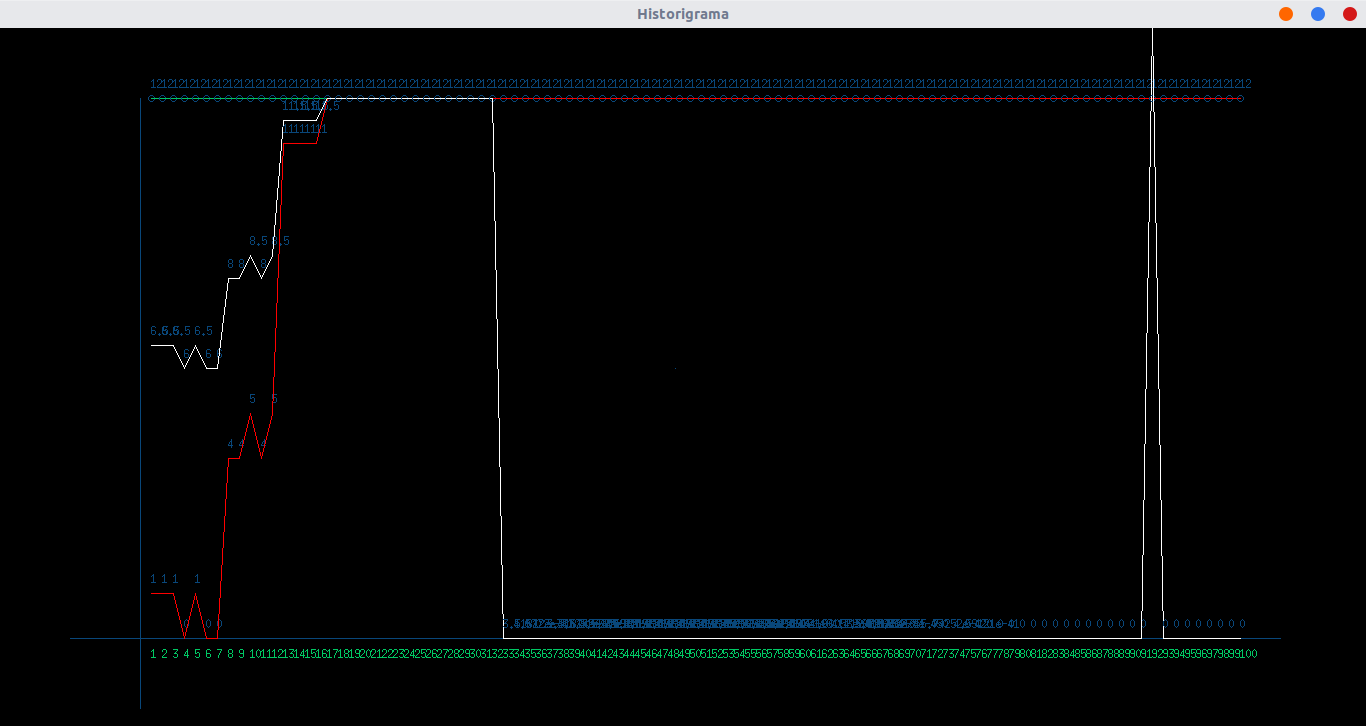
\includegraphics[scale=.3]{100gen}
\end{figure}
\section{Conclusión}
Este algoritmo es el algoritmo genético más simple, pero el más popular. En esta práctica se usó la selección por tornepo, la cual puede seleccionar al individuo menos apto. Los individuos más aptos son los que tiene más probabilidad de ser seleccioandos.
\end{document}